\documentclass{bioinfo}
\copyrightyear{2013}
\pubyear{2013}

\begin{document}
\firstpage{1}

\title[iview]{iview: WebGL Visualizer of Protein-Ligand Complex}
\author[Hongjian Li \textit{et~al}]{Hongjian Li\,$^{1,}$\footnote{to whom correspondence should be addressed}, Kwong-Sak Leung\,$^{1}$, Takanori Nakane\,$^{2}$ and Man-Hon Wong\,$^{1}$}
\address{$^{1}$Department of Computer Science and Engineering, Chinese University of Hong Kong, Hong Kong\\
$^{2}$Graduate School of Medicine, Kyoto University, Japan}

\history{Received on XXXXX; revised on XXXXX; accepted on XXXXX}

\editor{Associate Editor: XXXXXXX}

\maketitle

\begin{abstract}

\section{Motivation:}
Visualization of protein-ligand complex plays an important role in elaborating protein-ligand interactions and aiding novel drug design. Most existing web visualizers are either too complicated to use, or lack virtual reality support. The vital feature of macromolecular surface construction is also unavailable.

\section{Results:}
We have developed iview, an easy-to-use interactive WebGL visualizer of protein-ligand complex. It features three special effects in virtual reality settings, namely anaglyph, parallax barrier and oculus rift. It supports four surface representations including Van der Waals surface, solvent excluded surface, solvent accessible surface and molecular surface. Moreover, based on the feature-rich version of iview, we have also developed a neat and tailor-made version specifically for our istar web platform for protein-ligand docking purpose. This demonstrates the excellent portability of iview.

\section{Availability:}
http://istar.cse.cuhk.edu.hk/iview

\section{Contact:} \href{JackyLeeHongJian@Gmail.com}{JackyLeeHongJian@Gmail.com}, \href{nakane.t@gmail.com}{nakane.t@gmail.com}
\end{abstract}

\section{Introduction}

Visualization of protein-ligand complex plays an important role in elaborating protein-ligand interactions and aiding novel drug design. To date, dozens of visualization tools already exist. VMD \citep{1220}, PyMOL \citep{1221} and Chimera \citep{1219} are very well-known and highly cited. They can interpret multiple file formats and generate multiple representations to supply precise and powerful control. AutoDockTools4 \citep{596} provides native support for the PDBQT file format, which is widely used in various protein-ligand docking software such as AutoDock \citep{596}, AutoDock Vina \citep{595}, and our idock \citep{1153}. We also developed our own method \citep{1265} to visualize structures in virtual reality settings and employ fragment-based \textit{de novo} ligand design strategy for interactive drug design. PoseView \citep{748} and LigPlot+ \citep{951}, on the other hand, plot 2D diagrams of protein-ligand interactions from 3D coordinates.

In addition, there are web visualizers based on either Java applet, Adobe Flash, or HTML5 canvas. Jmol (http://www.jmol.org), an open source Java viewer for chemical structures in 3D, has been deployed worldwide and recognized as the \textit{de facto} molecular viewer on the web. JSmol \citep{1314}, a JavaScript-only version of Jmol, includes the full implementation of the entire set of Jmol functionalities. Although Jmol and JSmol support a large set of advanced features including scripting, they are too complicated for normal users. GLmol (http://webglmol.sourceforge.jp), a molecular viewer on WebGL/JavaScript using the three.js library, supports multiple file formats and representations, and features an experimental version of surface construction based on the EDTSurf algorithm \citep{1297,1350}, but it lacks virtual reality support. Another study \citep{1262} also presents a WebGL technology for rendering molecular surface using the SpiderGL library \citep{1320}. ChemDoodle Web Components (http://web.chemdoodle.com), a pure JavaScript chemical graphics and cheminformatics library, presents 2D and 3D graphics and animations for chemical structures, reactions and spectra, but it lacks protein surface construction.

Surface representation is a convenient way to visualize protein-ligand interactions. However, macromolecular surface calculation is computationally and memory intensive. Furthermore, the calculated mesh is very complex, often exceeding 500,000 polygons. Therefore its implementation in JavaScript/WebGL was considered to be very difficult. Most existing web visualizers are either too complicated to use, or lack virtual reality support. Moreover, the vital feature of protein surface construction is usually unavailable.

To address the above obstacles, we were inspired by ChemDoodle Web Components and GLmol, and have thus developed iview, an easy-to-use interactive WebGL visualizer of protein-ligand complex, featuring three special effects in virtual reality settings and four surface representations (Table S1). Furthermore, we show that iview can be easily modified to adapt to different applications. As an application example, we have recently developed a web platform called istar to automate large-scale protein-ligand docking using our idock \citep{1153}. Refactored from the feature-rich version of iview, we have also developed a neat and tailor-made version specifically for visualizing docking input data and output results of user-submitted jobs.

\begin{methods}
\section{Methods}

iview is refactored from GLmol 0.47, using three.js as its primary 3D engine with antialiasing support. It is based on WebGL canvas and can be easily integrated into existing HTML5 web pages to display molecular models without requiring Java or browser plugins. It loads a protein-ligand structure from the PDB (Protein Data Bank) \citep{539,537} as its data source via a RESTful interface. It renders four standard representations of primary structure, namely line, stick, ball \& stick and sphere, and five standard representations of secondary structure, namely ribbon, strand, cylinder \& plate, C alpha trace and B factor tube. It colors the structure by either atom spectrum, protein chain, protein secondary structure, B factor, residue name, residue polarity, or atom type, by setting the vertex colors of the geometry object of the corresponding representation. It supports user interactions including rotation, translation, zooming and slab with mouse or hand touch manipulation. It provides both perspective and orthographic cameras, and anaglyph, parallax barrier and oculus rift effects from three.js examples for use in a virtual reality environment. When users wear a spectacle with special filters on both sides, the disparity between two superimposed molecules creates a perception of depth, leading to visually more appealing identification of intermolecular interactions (Fig. S1).

We have ported EDTSurf \citep{1297,1350}, an fast algorithm to generating triangulated macromolecular surfaces by Euclidean distance transform, to JavaScript and integrated it into iview to construct and render in real time four representations of protein surface, namely Van der Waals surface, solvent excluded surface, solvent accessible surface and molecular surface, with opacity and wireframe adjustable by users (Fig. \ref{fig:4MBS}). Although the JavaScript implementation of the EDTSurf algorithm typically consumes a few seconds and 500MB to 700MB memory for computation, it is sufficiently efficient for practical applications. To limit CPU and memory usage, the calculation grid size is restricted to 180 x 180 x 180.

\begin{figure}[t]
\centerline{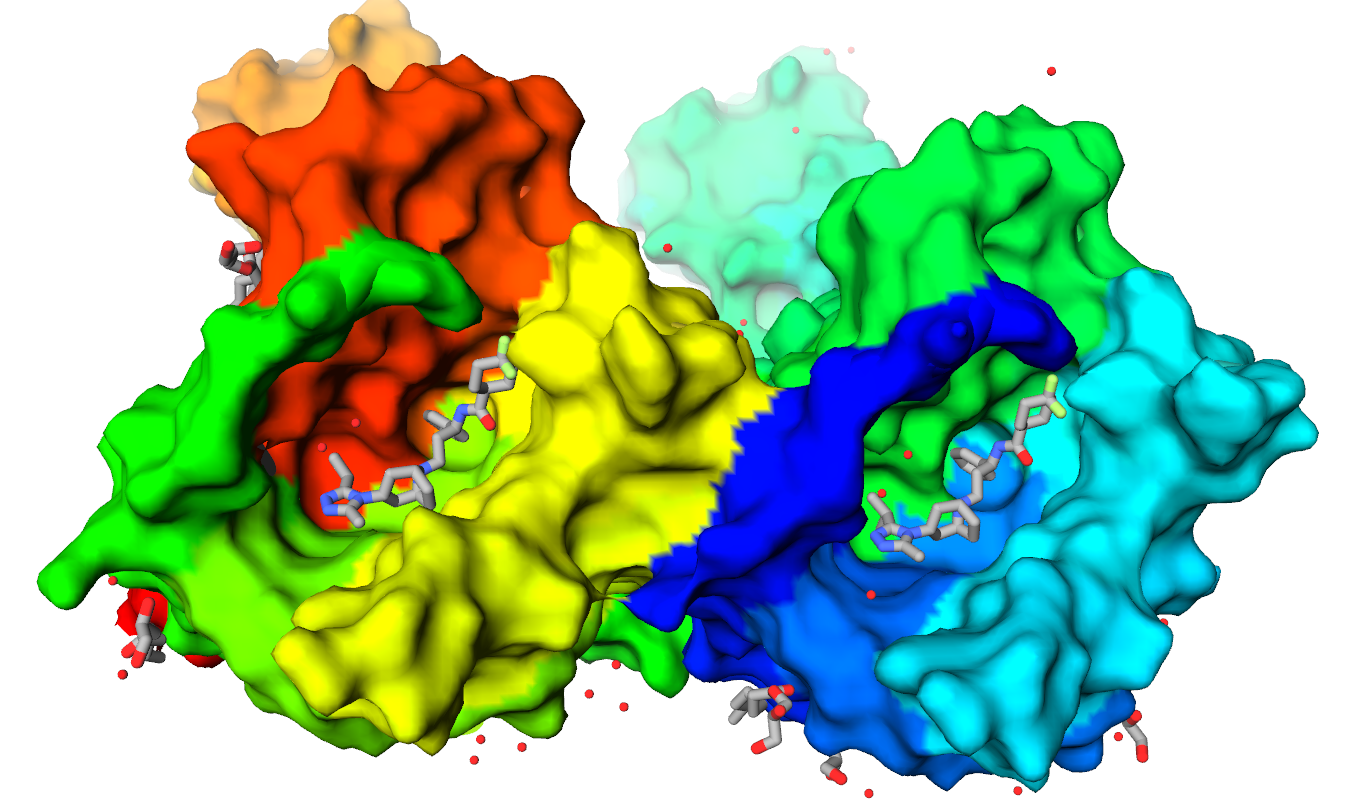
\includegraphics[width=\linewidth]{4MBS.png}}
\caption{iview rendering of the CCR5 chemokine receptor-HIV entry inhibitor maraviroc complex \citep{1348} (PDB code: 4MBS). The human CCR5 is rendered as molecular surface colored by spectrum. The marketed HIV drug maraviroc is rendered as stick colored by atom types. It can be clearly seen that the CCR5 forms a deep allosteric cavity where maraviroc is buried.}\label{fig:4MBS}
\end{figure}

We have successfully tested iview in Chrome 30, Firefox 25, Safari 6.1 and Opera 17. Support for IE 11 is experimental.

\subsection*{Application Example}
We emphasize portability and usability, and illustrate that iview can be easily modified to suit one's particular application, given that iview is free and open source under a permissive license. We take protein-ligand docking as an example. Based on the feature-rich version of iview, our tailor-made version specifically for idock jobs cleans up many dispensable functions, enabling a very neat interface. It only retains the rendering of primary structure of protein and ligand, as well as the construction of protein surface. Most importantly, it implements additional features especially for protein-ligand docking purpose.

In the input phase of a docking job, it merely requires a PDB file, which can be obtained either from the PDB database \citep{539,537} or via homology modeling, and then constructs the protein surface asynchronously in a separate web worker to keep the web page responsive. It automatically detects a binding site from the largest co-crystallized ligand first by finding the smallest cubic box that covers the entire ligand and then by extending the box by 50\% in all the three dimensions in order to reserve space for conformational sampling. In case of non-existence of co-crystallized ligand, the binding site is defaulted to the geometric center of the protein. The binding site is visually depicted in the form of a cubic box whose center and size can be manually adjusted by users in real time.

In the output phase of a docking job, it displays the user-supplied cubic box for users to confirm the predicted ligand conformations do fall inside the desired binding site. Other than PDB format, its parsers are capable of parsing a protein and multiple top hit ligands in PDBQT format used by idock. It displays the top hit ligand IDs in a horizontally scrollable row and provides a straightforward way to switch ligands easily through a button group. It has built-in support for putative intermolecular hydrogen bond detection by finding hydrogen bond donors and acceptors from protein and ligand and setting the distance threshold to 3.5\AA. It lists the docking result files, predicted free energy and binding affinity values, molecular properties, SMILES representation, compound suppliers and annotations, and putative hydrogen bond positions and their lengths, in order to give users a quick overview of the top hit ligands and assist them in making decisions of which compounds to purchase for subsequent wet-lab experiments (Fig. S2).

\end{methods}

\bibliographystyle{natbib}
%\bibliographystyle{achemnat}
%\bibliographystyle{plainnat}
%\bibliographystyle{abbrv}
%\bibliographystyle{bioinformatics}
%
%\bibliographystyle{plain}

\bibliography{../refworks}

\end{document}
